%\documentclass[12pt]{article}
%\usepackage[a4paper, margin=1in]{geometry} 
%\usepackage{graphicx} 
%\usepackage{hyperref}
%\usepackage{float}
%\usepackage{multicol}
%\usepackage{multirow}
%\usepackage[font=small, labelfont=bf]{caption}
%\usepackage{amssymb}
%\usepackage{amsmath}
%
%\begin{document}

%
% Measures with multiple thresholds
%
\subsection{Measures with multiple thresholds}
The test data set needs to be sorted by scores, and then confusion matrices can be calculated for multiple threshold values.

%
% Example of making confusion matrices with multiple thresholds
%
\subsubsection*{Example of making confusion matrices with multiple thresholds}

\noindent
Test data set
\begin{table}[H]
\centering
\scriptsize
\begin{tabular}{|l|l|l|l|l|l|l|l|l|l|l|l|l|l|l|l|l|l|l|l|l|}
\hline
Label & N  & P & P  & N & N  & N & P  & P  & P  & N & P  & N & P  & P  & N  & N & P  & P  & N  & N \\ \hline
Score & 27 & 4 & 17 & 9 & 11 & 2 & 15 & 19 & 22 & 3 & 23 & 7 & 10 & 25 & 11 & 1 & 26 & 28 & 24 & 3 \\ \hline
\end{tabular}
\end{table}

\noindent
Sorted test data set
\begin{table}[H]
\centering
\scriptsize
\begin{tabular}{lllllllllllllllllllll}
\hline
\multicolumn{1}{|l|}{Label} & \multicolumn{1}{l|}{P}  & \multicolumn{1}{l|}{N}  & \multicolumn{1}{l|}{P}  & \multicolumn{1}{l|}{P}  & \multicolumn{1}{l|}{N}  & \multicolumn{1}{l|}{P}  & \multicolumn{1}{l|}{P}  & \multicolumn{1}{l|}{P}  & \multicolumn{1}{l|}{P}  & \multicolumn{1}{l|}{P}  & \multicolumn{1}{l|}{N}  & \multicolumn{1}{l|}{N}  & \multicolumn{1}{l|}{P}  & \multicolumn{1}{l|}{N} & \multicolumn{1}{l|}{N} & \multicolumn{1}{l|}{P} & \multicolumn{1}{l|}{N} & \multicolumn{1}{l|}{N} & \multicolumn{1}{l|}{N} & \multicolumn{1}{l|}{N} \\ \hline
\multicolumn{1}{|l|}{Score} & \multicolumn{1}{l|}{28} & \multicolumn{1}{l|}{27} & \multicolumn{1}{l|}{26} & \multicolumn{1}{l|}{25} & \multicolumn{1}{l|}{24} & \multicolumn{1}{l|}{23} & \multicolumn{1}{l|}{22} & \multicolumn{1}{l|}{19} & \multicolumn{1}{l|}{17} & \multicolumn{1}{l|}{15} & \multicolumn{1}{l|}{11} & \multicolumn{1}{l|}{11} & \multicolumn{1}{l|}{10} & \multicolumn{1}{l|}{9} & \multicolumn{1}{l|}{7} & \multicolumn{1}{l|}{4} & \multicolumn{1}{l|}{3} & \multicolumn{1}{l|}{3} & \multicolumn{1}{l|}{2} & \multicolumn{1}{l|}{1} \\ \hline
\multirow{2}{*}{Threshold}  &                         &                         & \multicolumn{2}{c}{$\uparrow$}                             &                         &                         &                         &                         & \multicolumn{2}{c}{$\uparrow$}                             &                         &                         &                         &                        &                        & \multicolumn{2}{c}{$\uparrow$}                           &                        &                        &                        \\
                            &                         &                         & \multicolumn{2}{c}{1}                             &                         &                         &                         &                         & \multicolumn{2}{c}{2}                             &                         &                         &                         &                        &                        & \multicolumn{2}{c}{3}                           &                        &                        &                       
\end{tabular}
\end{table}

\noindent
1st threshold (score = 25.5)
\begin{table}[H]
\footnotesize
\begin{tabular}{|l|l|}
\hline
2 TPs & 1 FPs \\ \hline
8 FNs & 9 TNs \\ \hline
\end{tabular}
\end{table}

\noindent
2nd threshold (score = 16)
\begin{table}[H]
\footnotesize
\begin{tabular}{|l|l|}
\hline
7 TPs & 2 FPs \\ \hline
3 FNs & 8 TNs \\ \hline
\end{tabular}
\end{table}

\noindent
3rd threshold (score = 3.5)
\begin{table}[H]
\footnotesize
\begin{tabular}{|l|l|}
\hline
10 TPs & 6 FPs \\ \hline
0 FNs & 4 TNs \\ \hline
\end{tabular}
\end{table}

%
% ROC and precision-recall
%
\subsubsection*{ROC and precision-recall}
These measure are based on the confusion matrices of all possible threshold values.

\begin{itemize}
\item ROC (Receiver operating characteristic) plot
\item Precision-recall plot
\end{itemize}

\begin{figure}[H]
  \centering
      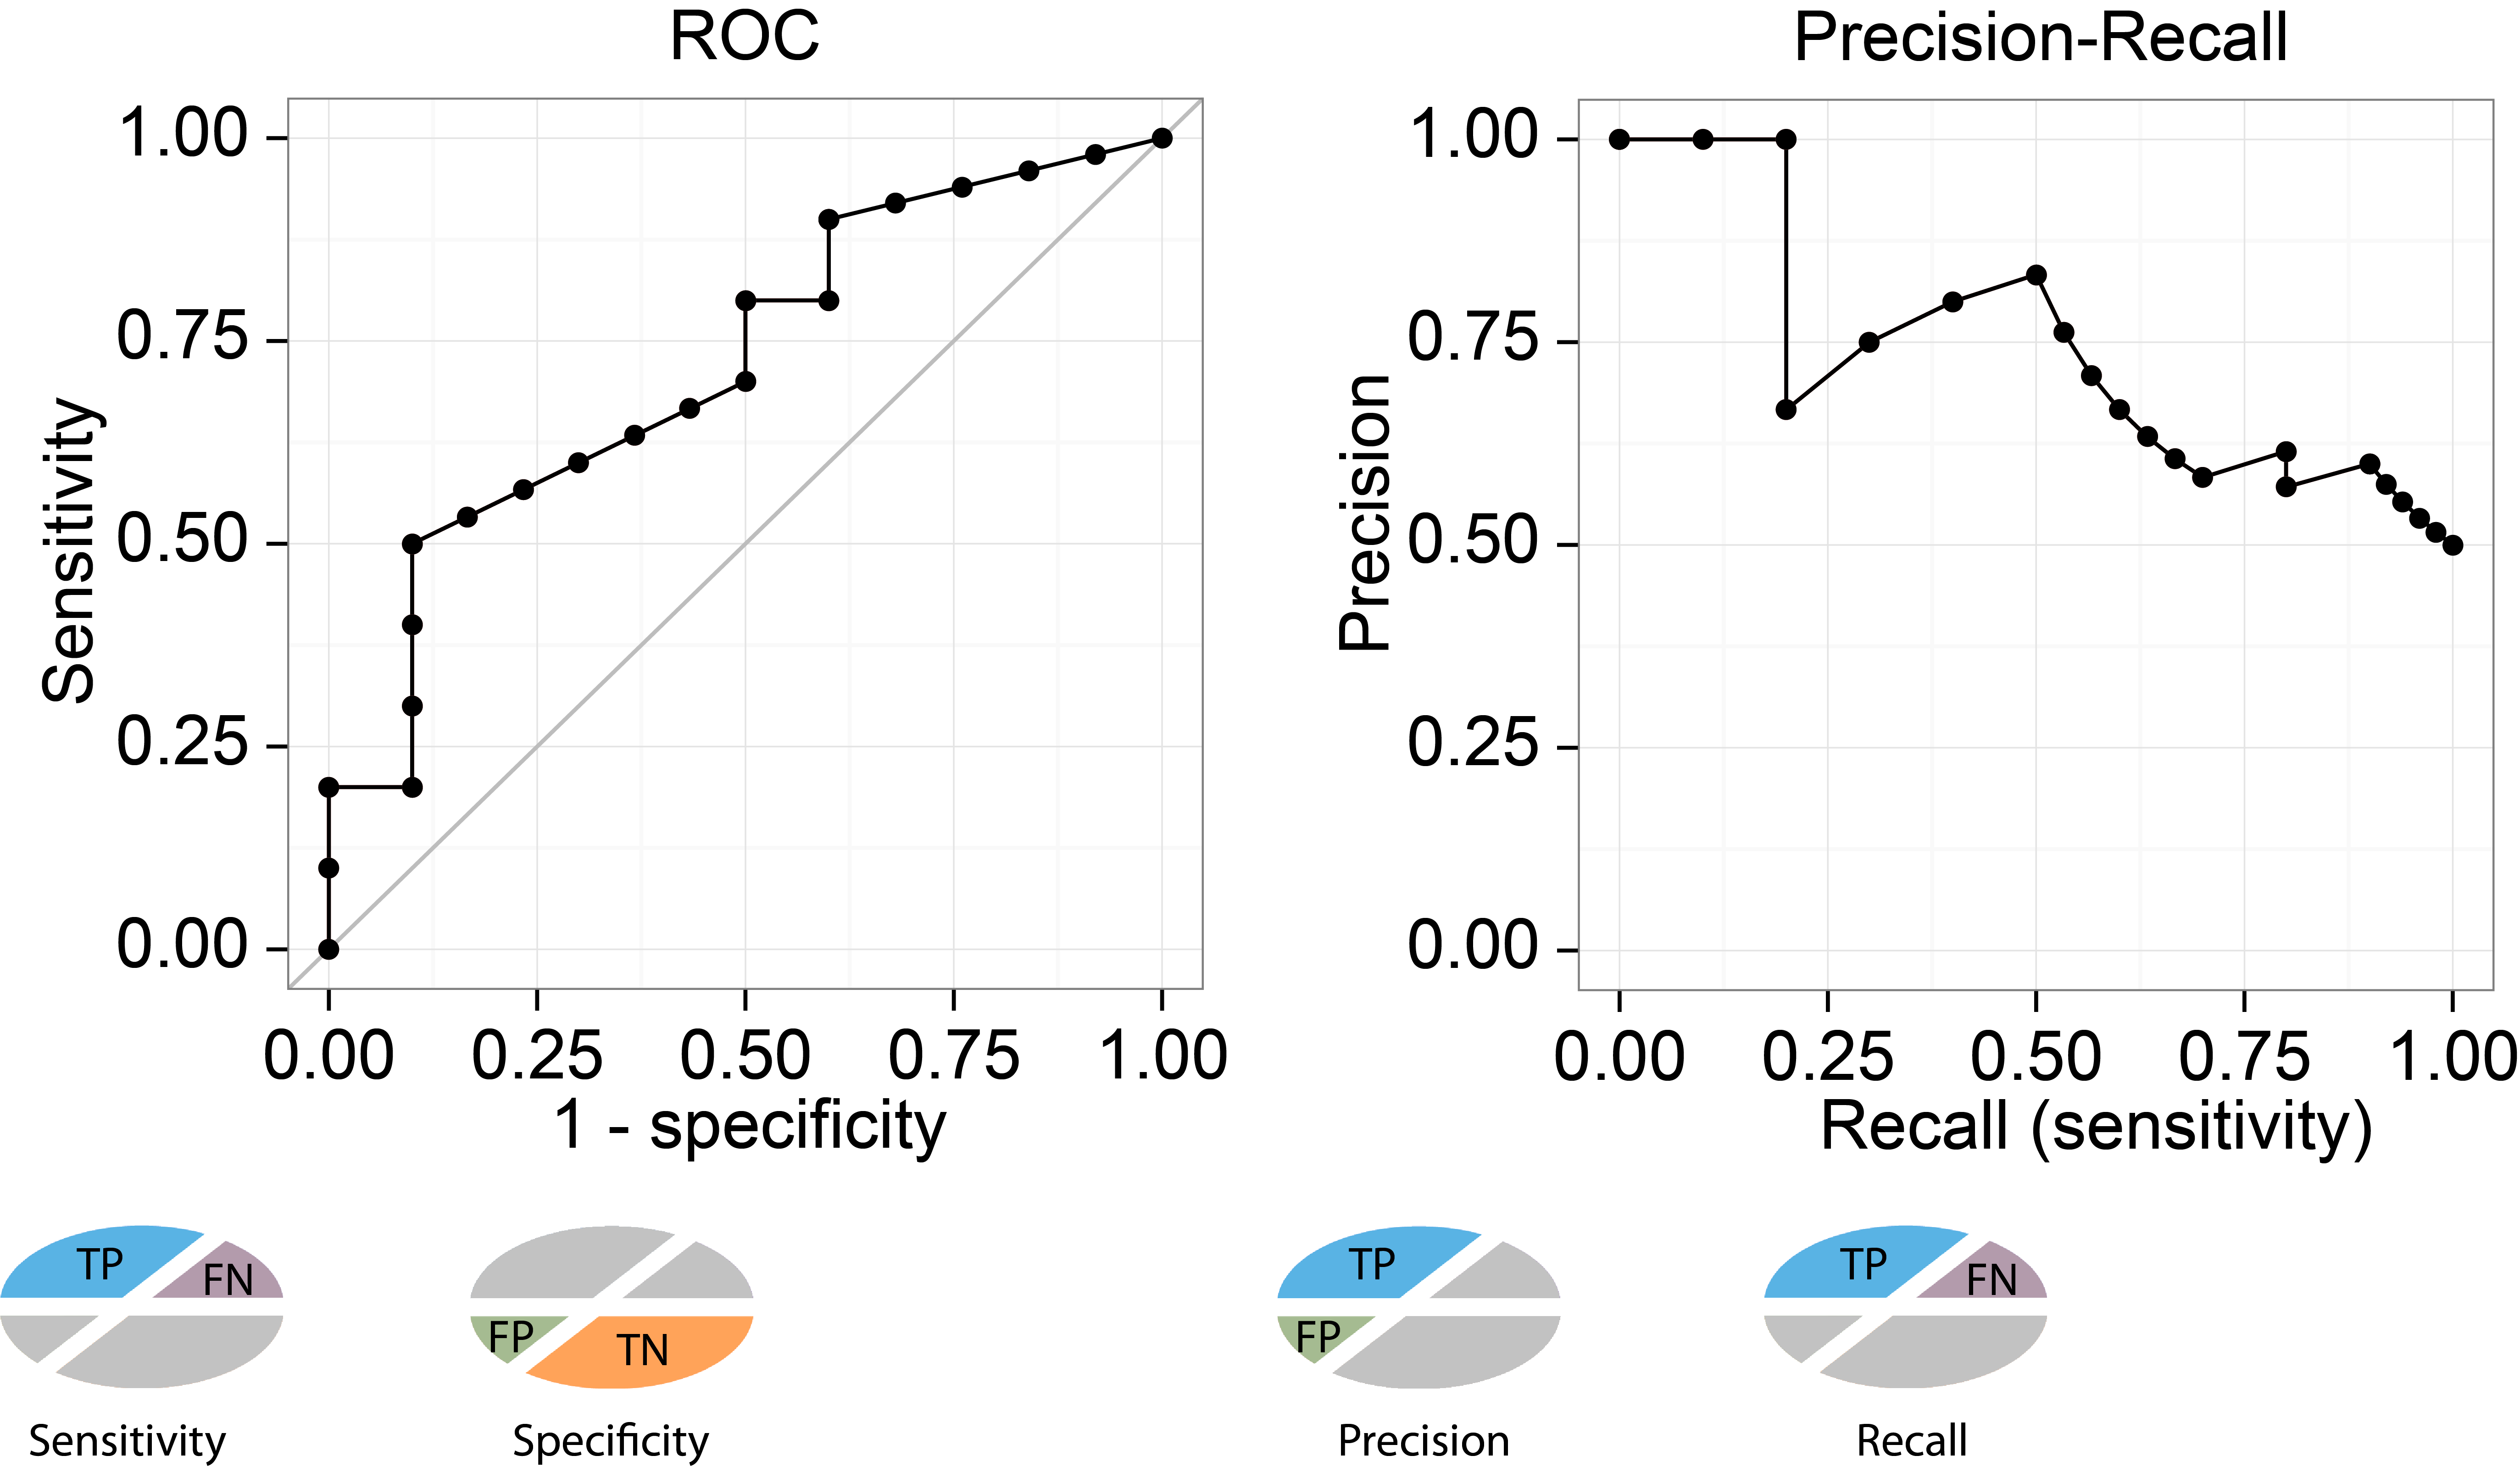
\includegraphics[width=0.6 \textwidth]{fig07/roc_precision-recall.png}
  \caption{ROC and precision-recall plots}
\end{figure}

%
% Exercise \thesection.1
%
\subsubsection*{Exercise \thesection.1}
Draw an ROC curve for the following specificity and sensitivity values.

\begin{table}[H]
\centering
\begin{tabular}{|l|l|l|l|}
\hline
Threshold & Specificity & 1 - Specificity & Sensitivity \\ \hline
10        & 1           & 0               & 0           \\ \hline
9         & 0.8         & 0.2             & 0.8         \\ \hline
8         & 0.6         & 0.4             & 0.8         \\ \hline
7         & 0.6         & 0.4             & 1           \\ \hline
6         & 0.4         & 0.6             & 1           \\ \hline
5         & 0.2         & 0.8             & 1           \\ \hline
4         & 0           & 1               & 1           \\ \hline
\end{tabular}
\end{table}

\begin{figure}[H]
  \centering
      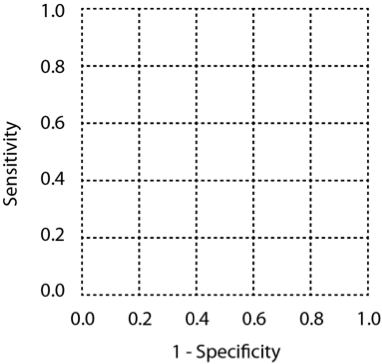
\includegraphics[width=0.4 \textwidth]{fig07/roc.png}
\end{figure}

\bigskip 

%\end{document}
